\documentclass[11pt,letterpaper]{article}
%graph pour image H
\usepackage{float}

%Highlight
\usepackage{soul}

%Pour vecteur unitaire
\newcommand{\uvec}[1]{\boldsymbol{\hat{\textbf{#1}}}}

% Pour Dessin
\usepackage{tikz}
\usepackage{amsmath}
\usepackage{mathrsfs}
\usetikzlibrary{arrows.meta, positioning}

% Pour Braket de Quantique
\usepackage{braket}

% Pour circle red
\usetikzlibrary{shapes,
tikzmark}
\tikzset{every tikzmarknode/.style={%
draw=red, semithick, inner sep=2pt}
}


% Pour box paragraph
\usepackage{fancybox,framed}

% packetages pour ecrire en français
\usepackage[french]{babel}
\usepackage[utf8]{inputenc}
\usepackage[T1]{fontenc}

% pour les maths, les graphiques et la navigation dans le pdf
\usepackage{amsmath, amssymb, mathtools, mathrsfs, bm, array, units, amsthm, dsfont}
\usepackage{graphicx,caption}
\graphicspath{{./}}
\usepackage{hyperref}
\hypersetup{
    pdftitle={De l'étalonnage à la traque du potassium-40: spectroscopie gamma avec un scintillateur NaI(Tl)},
    pdfauthor={L-F. Brodeur (LFBRO1), S. L-Tremblay (SILAT10)}
}
\usepackage{physics} %très utile pour ecrire plus rapidement des matrices, des derivees, etc. Allez voir la documentation!

% marges, police de caractère et header
\usepackage{geometry}
\geometry{top=30mm, bottom=30mm, left=20mm, right=20mm}
\usepackage{cochineal}
\usepackage{fancyhdr}
\pagestyle{fancy}

\parindent=0mm % pas d'indentation

\lhead{L-F. Brodeur (IDUL: LFBRO1) et S. L-Tremblay (IDUL: SILAT10)}
\rhead{Détecteurs de radiations nucléaires}
\fancyheadoffset{0 cm}

\setlength{\headheight}{13.6pt}

% commandes pour ecrire des equations plus vite avec leur label
\newcommand{\beq}[1]{\begin{equation} \label{#1}}
\def\enq{\end{equation}}

% C'est parti!
\begin{document}
\shorthandoff{;:!?}
\thispagestyle{empty} % pas de header sur la première page
\begin{center}

\noindent
\begin{minipage}[t]{0.5\textwidth}
\raggedright
{\large GPH-3000 \textit{Travaux pratiques avancés}}\\
{\large Automne 2026 $\vert$ GPH-3000 (Groupe: 85213)}
\end{minipage}%
\begin{minipage}[t]{0.5\textwidth}
\raggedleft
{\large \textsc{L-F. Brodeur (IDUL: LFBRO1)}}\\
{\large \textsc{S. L-Tremblay (IDUL: SILAT10)}}
\end{minipage}
\\~\\
\vspace{1em}
{\Large \textbf{De l'étalonnage à la traque du potassium-40:} } \\
{\Large \textbf{spectroscopie gamma avec un scintillateur NaI(Tl)} } \\[0.3em]
{\large Date d'expérimentation: 17 septembre 2026 \quad $\vert$ \quad Remis le \today}

\end{center}

\vspace{0.5em}
\subsection*{Résumé}
On ne le sent pas, mais des rayons gamma nous traversent en ce moment même: ils viennent du béton, des roches, et même de l'intérieur de notre propre corps. Cette expérience visait à étalonner un scintillateur NaI(Tl) couplé à un analyseur multicanaux (Easy-MCA-8k), à l'aide de cinq sources $\gamma$ connues (\textsuperscript{133}Ba, \textsuperscript{57}Co, \textsuperscript{60}Co, \textsuperscript{137}Cs, \textsuperscript{22}Na, onze raies de 30,85~keV à 1332,50~keV), puis à utiliser cet étalonnage pour identifier la source dominante du bruit de fond radioactif du laboratoire. Un modèle quadratique canal-énergie a été retenu ($R^2 = 0,99997$, RMSE $= 2,6~\text{keV}$, contre $5,0~\text{keV}$ pour un modèle linéaire), et la résolution du détecteur suit une loi de puissance $R = (122 \pm 15)\cdot E^{-0,44 \pm 0,03}~\%$, proche du comportement statistique attendu en $E^{-1/2}$. Sur le spectre du \textsuperscript{137}Cs, le front Compton et le pic de rétrodiffusion prédits par la cinématique de diffusion Compton (477,4~keV et 184,3~keV) coïncident, à la résolution du détecteur près, avec les structures observées ($\approx 462$~keV et $\approx 195$~keV). Enfin, une acquisition de 36~minutes sans source a révélé un pic dominant à $1485 \pm 3~\text{keV}$, compatible avec la raie de $1460,8~\text{keV}$ du \textsuperscript{40}K. Ceci confirme que le potassium naturel, présent dans le béton, la brique et nous-mêmes, est la principale source de radioactivité ambiante du laboratoire. Le même principe, étalonner un détecteur puis identifier une source à partir de son spectre, est utilisé en surveillance environnementale, en sécurité aux frontières et en médecine nucléaire.

\section{Introduction}

La radioactivité est présente presque partout dans notre environnement, mais elle reste imperceptible sans instrumentation. Depuis la découverte de la radioactivité par Becquerel en 1896, on sait que certains noyaux se désintègrent en émettant des rayonnements pénétrants. Un compteur Geiger permet de détecter qu'un rayon gamma est présent, mais il ne donne aucune information sur son énergie: tous les événements produisent le même signal. Un scintillateur, lui, produit un signal dont l'amplitude est proportionnelle à l'énergie du photon incident, ce qui permet d'identifier l'isotope qui l'a émis.

L'objectif de cette expérience était double. D'abord, étalonner un scintillateur à l'iodure de sodium (NaI(Tl)) à l'aide de cinq sources $\gamma$ d'énergies connues, afin de convertir la sortie brute de l'électronique (un numéro de canal) en une grandeur physique utile (une énergie en keV). Ensuite, utiliser cet instrument fraîchement calibré pour répondre à une question concrète: quelle est la source de la radioactivité ambiante mesurée dans le laboratoire, en l'absence de toute source radioactive volontairement introduite?

Le présent rapport est organisé comme suit. La section~2 rappelle brièvement les mécanismes d'interaction d'un rayon gamma avec la matière (essentiels pour interpréter la forme des spectres) et le principe de fonctionnement du scintillateur. La section~3 décrit le montage et la procédure d'analyse. La section~4 présente les résultats: la courbe d'étalonnage, l'anatomie détaillée d'un spectre (avec une attention particulière portée au front Compton et au pic de rétrodiffusion), la résolution en énergie du détecteur, et l'identification de la raie dominante du bruit de fond. La section~5 discute la qualité de ces résultats et leurs limites, avant une conclusion.

\section{Théorie}

\subsection{Interaction des rayons gamma avec la matière}

Un rayon gamma qui traverse le cristal de NaI(Tl) peut y déposer son énergie de trois façons \cite{knoll}. Sous $\sim$1~MeV, le régime qui nous concerne ici à l'exception des deux raies du \textsuperscript{60}Co, deux processus dominent:

\begin{itemize}
    \item \emph{L'effet photoélectrique}: le photon cède \emph{toute} son énergie à un électron du cristal, qui l'absorbe complètement. C'est ce processus qui produit le \emph{photopic}, c'est-à-dire le pic étroit correspondant à l'énergie exacte du rayon gamma incident.
    \item \emph{La diffusion Compton}: le photon ne cède qu'une partie de son énergie à un électron quasi libre et continue sa route, dévié, avec une énergie moindre. L'énergie transférée à l'électron dépend de l'angle de diffusion $\theta$ et varie continûment entre 0 (diffusion vers l'avant) et un maximum (diffusion à $180^\circ$). C'est ce qui produit le \emph{continuum Compton}, un plateau qui s'étend sous le photopic.
\end{itemize}

L'énergie maximale qu'un électron peut recevoir par diffusion Compton, correspondant à une rétrodiffusion à $180^\circ$, définit le \emph{front Compton}:
\beq{eq:compton_edge}
    E_C = \frac{2E_\gamma^2}{m_e c^2 + 2E_\gamma} ,
\enq
où $E_\gamma$ est l'énergie du photon incident et $m_e c^2 = 511~\text{keV}$ l'énergie de masse au repos de l'électron. Au-delà de $E_C$, aucun événement Compton simple ne peut déposer plus d'énergie dans le cristal. C'est pourquoi le continuum chute abruptement à cette énergie.

Un second artefact, moins souvent discuté, est le \emph{pic de rétrodiffusion}. Un photon peut se diffuser Compton \emph{à $180^\circ$ dans le blindage ou les matériaux environnant le détecteur} (table, boîtier de la source, etc.) avant d'entrer dans le cristal, où il est alors absorbé par effet photoélectrique. L'énergie qu'il dépose correspond au complément de $E_C$:
\beq{eq:backscatter}
    E_{bs} = E_\gamma - E_C = \frac{E_\gamma}{1 + 2E_\gamma / (m_e c^2)} .
\enq
Ce pic apparaît donc sous forme d'une bosse dans le continuum, juste en deçà du front Compton.

Au-dessus de $1,022~\text{MeV}$ ($= 2 m_e c^2$), un troisième mécanisme, la production de paires électron-positon, devient possible mais reste négligeable dans nos spectres, dont l'énergie maximale (1332,5~keV, \textsuperscript{60}Co) est trop proche du seuil pour que ce processus contribue de façon mesurable.

\subsection{Le scintillateur NaI(Tl) et la chaîne de détection}

Le cristal de NaI dopé au thallium émet une brève scintillation lumineuse (temps de désexcitation $\approx 0,25~\mu\text{s}$) chaque fois qu'un photon $\gamma$ y dépose de l'énergie, avec un nombre de photons de scintillation proportionnel à cette énergie déposée \cite{protocole}. Un tube photomultiplicateur convertit cette lumière en une impulsion électrique, elle-même mise en forme par un préamplificateur puis un amplificateur. L'analyseur multicanaux (MCA) classe ensuite chaque impulsion selon son amplitude dans l'un de ses 4096 canaux, construisant ainsi un histogramme (le spectre) du nombre de photons détectés en fonction du canal. La relation entre le numéro de canal et l'énergie déposée dépend du gain de l'électronique et doit être établie empiriquement: c'est l'objet de l'étalonnage.

\subsection{Radioactivité ambiante}

Même en l'absence de toute source radioactive « volontaire », un détecteur $\gamma$ enregistre toujours un signal. Ce bruit de fond provient à la fois du rayonnement cosmique et de la radioactivité naturelle présente dans notre environnement immédiat: les matériaux de construction (béton, brique, granite) contiennent des traces d'éléments radioactifs à longue durée de vie, principalement le \textsuperscript{40}K et les descendants des chaînes de désintégration de l'\textsuperscript{238}U et du \textsuperscript{232}Th. Le \textsuperscript{40}K est particulièrement intéressant: il représente environ 0,012~\% du potassium naturel, a une demi-vie de 1,25 milliard d'années, et se désintègre 11~\% du temps par capture électronique vers un état excité du \textsuperscript{40}Ar, lequel se désexcite en émettant un photon $\gamma$ à 1460,8~keV \cite{nndc}. Le potassium étant abondant dans le corps humain, les os et les matériaux de construction, cette raie est presque toujours la signature dominante du bruit de fond ambiant dans un laboratoire universitaire.

\section{Méthodologie}

\subsubsection*{Montage}
La chaîne d'acquisition (Figure~\ref{fig:montage}) est celle décrite au protocole \cite{protocole}: une source scellée est placée devant un scintillateur NaI(Tl) couplé à un tube photomultiplicateur. Le signal passe par un préamplificateur puis un amplificateur avant d'être numérisé par un analyseur multicanaux Easy-MCA-8k (PHY-0040-AA), relié à un ordinateur et piloté par le logiciel Maestro (v7.01). Le gain de l'amplificateur a été fixé une fois pour toutes en début de séance, comme le recommande le protocole, et n'a plus été retouché par la suite. Il s'agit d'une précaution essentielle, puisque tout changement de gain invaliderait l'étalonnage.

\begin{figure}[H]
    \centering
    \begin{tikzpicture}[
        node distance=6mm and 8mm,
        block/.style={draw, rounded corners, align=center, minimum height=1.1cm, minimum width=2.1cm, font=\small},
        arrow/.style={-{Latex[length=2mm]}, thick}
    ]
        \node[block] (source) {Source\\$\gamma$};
        \node[block, right=of source] (nai) {NaI(Tl)\\+ PM};
        \node[block, right=of nai] (preamp) {Préampli-\\ficateur};
        \node[block, right=of preamp] (amp) {Amplifi-\\cateur};
        \node[block, right=of amp] (mca) {MCA\\Easy-MCA-8k};
        \node[block, right=of mca] (pc) {Ordinateur\\(Maestro)};
        \draw[arrow] (source) -- (nai);
        \draw[arrow] (nai) -- (preamp);
        \draw[arrow] (preamp) -- (amp);
        \draw[arrow] (amp) -- (mca);
        \draw[arrow] (mca) -- (pc);
    \end{tikzpicture}
    \caption{Chaîne d'acquisition du scintillateur: le signal lumineux de la scintillation, converti en impulsion électrique par le tube photomultiplicateur, est mis en forme puis numérisé par le MCA avant d'être histogrammé par ordinateur.}
    \label{fig:montage}
\end{figure}

\subsubsection*{Étalonnage}
Cinq sources scellées (\textsuperscript{133}Ba, \textsuperscript{57}Co, \textsuperscript{60}Co, \textsuperscript{137}Cs, \textsuperscript{22}Na) ont été acquises individuellement, fournissant onze raies $\gamma$ de référence réparties entre 30,85~keV et 1332,50~keV (Tableau~\ref{tab:acquisitions}). Chaque source a été placée devant le détecteur pour un temps d'acquisition suffisant pour obtenir un photopic net (de 3 à 11~minutes selon l'activité de la source), tandis qu'une acquisition beaucoup plus longue (36~minutes) a été faite sans aucune source, pour caractériser le bruit de fond, conformément à la recommandation du protocole de faire cette longue acquisition en parallèle des autres manipulations \cite{protocole}.

\subsubsection*{Analyse}
L'ensemble du traitement a été fait en Python (NumPy/SciPy), voir le script \texttt{analyse\_spectres.py} du dépôt du cours. Pour chaque raie de référence, la région du spectre autour du canal attendu est d'abord localisée par une recherche de maximum local, puis ajustée par une gaussienne sur fond linéaire,
\beq{eq:gauss}
    N(x) = A \exp\!\left[-\frac{(x-\mu)^2}{2\sigma^2}\right] + mx + b ,
\enq
par moindres carrés non linéaires (\texttt{scipy.optimize.curve\_fit}), ce qui donne le centroïde $\mu$ (canal), son incertitude statistique $\Delta\mu$ (tirée de la matrice de covariance de l'ajustement) et la largeur à mi-hauteur $\text{FWHM} = 2,3548\,\sigma$. Les onze couples (canal, énergie) sont ensuite utilisés pour ajuster une relation d'étalonnage $E(\text{canal})$, à la fois linéaire et quadratique. Le modèle quadratique n'est retenu que s'il réduit sensiblement l'erreur quadratique moyenne (RMSE), pour éviter de sur-ajuster onze points avec un paramètre superflu. Un point important: plutôt que de tracer le nombre de coups bruts, tous les spectres sont présentés en taux de comptage (coups/s), obtenus en divisant par le \emph{temps vif} (« live time ») rapporté par le MCA plutôt que par le temps réel écoulé. Le temps vif exclut automatiquement les intervalles où l'électronique était occupée à traiter une impulsion précédente (temps mort). Cette normalisation corrige donc directement pour le temps mort sans calcul supplémentaire, ce qui est particulièrement important pour la source de \textsuperscript{137}Cs, dont le taux de comptage élevé a occasionné une fraction de temps mort de 22~\% (Tableau~\ref{tab:acquisitions}).

\begin{table}[htbp]
\centering
\caption{Sources utilisées, raies de référence et statistiques d'acquisition. Le temps vif est celui utilisé pour normaliser les spectres (taux de comptage). La fraction de temps mort quantifie l'écart entre temps réel et temps vif.}
\label{tab:acquisitions}
\small
\begin{tabular}{lccc}
\hline
Source & Raies utilisées (keV) & Temps vif / réel (s) & Temps mort (\%) \\
\hline
\textsuperscript{133}Ba & 30,85 / 81,00 / 302,85 / 356,02 & 372 / 383 & 2,9 \\
\textsuperscript{57}Co  & 122,06 & 675 / 687 & 1,7 \\
\textsuperscript{60}Co  & 1173,20 / 1332,50 & 896 / 909 & 1,4 \\
\textsuperscript{137}Cs & 32,00\textsuperscript{a} / 661,70 & 180 / 232 & 22,4 \\
\textsuperscript{22}Na  & 511,00 / 1274,50 & 186 / 196 & 5,1 \\
Bruit de fond & aucune (identification a posteriori) & 2155 / 2157 & 0,1 \\
\hline
\end{tabular}
\\[0.3em]
{\footnotesize \textsuperscript{a} Raie X caractéristique du baryum (transition K), et non une désexcitation nucléaire du \textsuperscript{137}Cs lui-même.}
\end{table}

\section{Résultats}

\subsection{Étalonnage en énergie}

La Figure~\ref{fig:calib} montre les onze points d'étalonnage ainsi que les modèles linéaire et quadratique. Le modèle quadratique,
\beq{eq:calib}
    E(\text{canal}) = (4,515 \times 10^{-6})\,\text{canal}^2 + 0,3902\,\text{canal} - 3,01~\text{keV} ,
\enq
réduit l'erreur quadratique moyenne de $5,0~\text{keV}$ (modèle linéaire) à $2,6~\text{keV}$ ($R^2 = 0,99997$), une amélioration suffisamment nette pour être retenue plutôt que d'ajouter un paramètre libre sans bénéfice réel. Cette légère composante quadratique est un effet bien documenté de non-linéarité de la réponse du couple scintillateur/photomultiplicateur, particulièrement visible aux basses énergies \cite{knoll}. Le Tableau~\ref{tab:peaks} détaille chaque raie individuellement.

\begin{figure}[H]
    \centering
    
\includegraphics[width=0.56\textwidth]{../figures/01_calibration.png}
    \caption{Étalonnage du scintillateur: énergie (littérature) en fonction du canal ajusté, pour les onze raies des cinq sources. Le panneau du bas montre les résidus par rapport au modèle quadratique retenu. Ils demeurent compatibles avec le RMSE global de 2,6~keV, sans tendance systématique évidente d'une source à l'autre.}
    \label{fig:calib}
\end{figure}

\begin{table}[htbp]
\centering
\caption{Détail des onze raies d'étalonnage: énergie de référence, canal ajusté, résidu par rapport au modèle quadratique, et résolution en énergie ($R = \text{FWHM}/E$).}
\label{tab:peaks}
\footnotesize
\begin{tabular}{lccccc}
\hline
Source & $E_{\text{lit.}}$ (keV) & Canal & Résidu (keV) & FWHM (keV) & $R$ (\%) \\
\hline
\textsuperscript{133}Ba & 30,85  & $82,15 \pm 0,05$   & $-1,8$ & 8,1  & 27,7 \\
\textsuperscript{133}Ba & 81,00  & $220,70 \pm 0,08$  & $+2,3$ & 12,6 & 15,1 \\
\textsuperscript{133}Ba & 302,85 & $780,71 \pm 1,52$  & $+1,5$ & 25,6 & 8,4  \\
\textsuperscript{133}Ba & 356,02 & $920,93 \pm 0,93$  & $+4,1$ & 42,1 & 11,7 \\
\textsuperscript{57}Co  & 122,06 & $319,16 \pm 0,05$  & $-0,1$ & 16,2 & 13,3 \\
\textsuperscript{60}Co  & 1173,20& $2909,89 \pm 5,20$ & $-2,6$ & 61,6 & 5,3  \\
\textsuperscript{60}Co  & 1332,50& $3296,26 \pm 7,73$ & $-0,3$ & 66,8 & 5,0  \\
\textsuperscript{137}Cs & 32,00  & $83,14 \pm 0,07$   & $-2,5$ & 9,9  & 33,7 \\
\textsuperscript{137}Cs & 661,70 & $1659,48 \pm 0,40$ & $-4,8$ & 57,8 & 8,8  \\
\textsuperscript{22}Na  & 511,00 & $1299,96 \pm 1,40$ & $+0,8$ & 54,5 & 10,7 \\
\textsuperscript{22}Na  & 1274,50& $3166,48 \pm 7,07$ & $+3,3$ & 57,9 & 4,5  \\
\hline
\end{tabular}
\end{table}

\subsection{Anatomie d'un spectre: effet photoélectrique, diffusion Compton et rétrodiffusion}

Le spectre du \textsuperscript{137}Cs (Figure~\ref{fig:compton}) est particulièrement instructif parce que la source n'émet essentiellement qu'une seule raie $\gamma$ (661,7~keV). Toutes les structures observées sous le photopic proviennent donc de la physique de l'interaction gamma-matière, et non d'un mélange de plusieurs énergies. On y distingue nettement:
\begin{itemize}
    \item le \emph{photopic} à 661,7~keV (effet photoélectrique, Tableau~\ref{tab:peaks}).
    \item un \emph{plateau Compton} entre $\sim 50$ et $\sim 430$~keV, relativement plat comme attendu pour une diffusion à petit angle sur des électrons quasi libres.
    \item une \emph{chute abrupte} du continuum, dont le point mi-hauteur se situe à $\approx 462~\text{keV}$, en bon accord avec le front Compton théorique de $477,4~\text{keV}$ (éq.~\ref{eq:compton_edge}) compte tenu de la résolution du détecteur à cette énergie (d'environ 8 à 9~\%, soit un $\text{FWHM}$ d'environ 40~keV). L'écart de 15~keV est donc inférieur à une demi-largeur à mi-hauteur.
    \item une \emph{bosse de rétrodiffusion} centrée vers $\approx 195~\text{keV}$, cohérente avec la prédiction de $184,3~\text{keV}$ (éq.~\ref{eq:backscatter}) à la résolution près.
\end{itemize}
On note aussi un pic étroit à 32,0~keV, trop bas en énergie pour être un photopic Compton. Il s'agit de la raie X caractéristique du baryum (produit de désintégration du \textsuperscript{137}Cs), émise lors du réarrangement électronique qui suit la désexcitation nucléaire.

\begin{figure}[H]
    \centering
    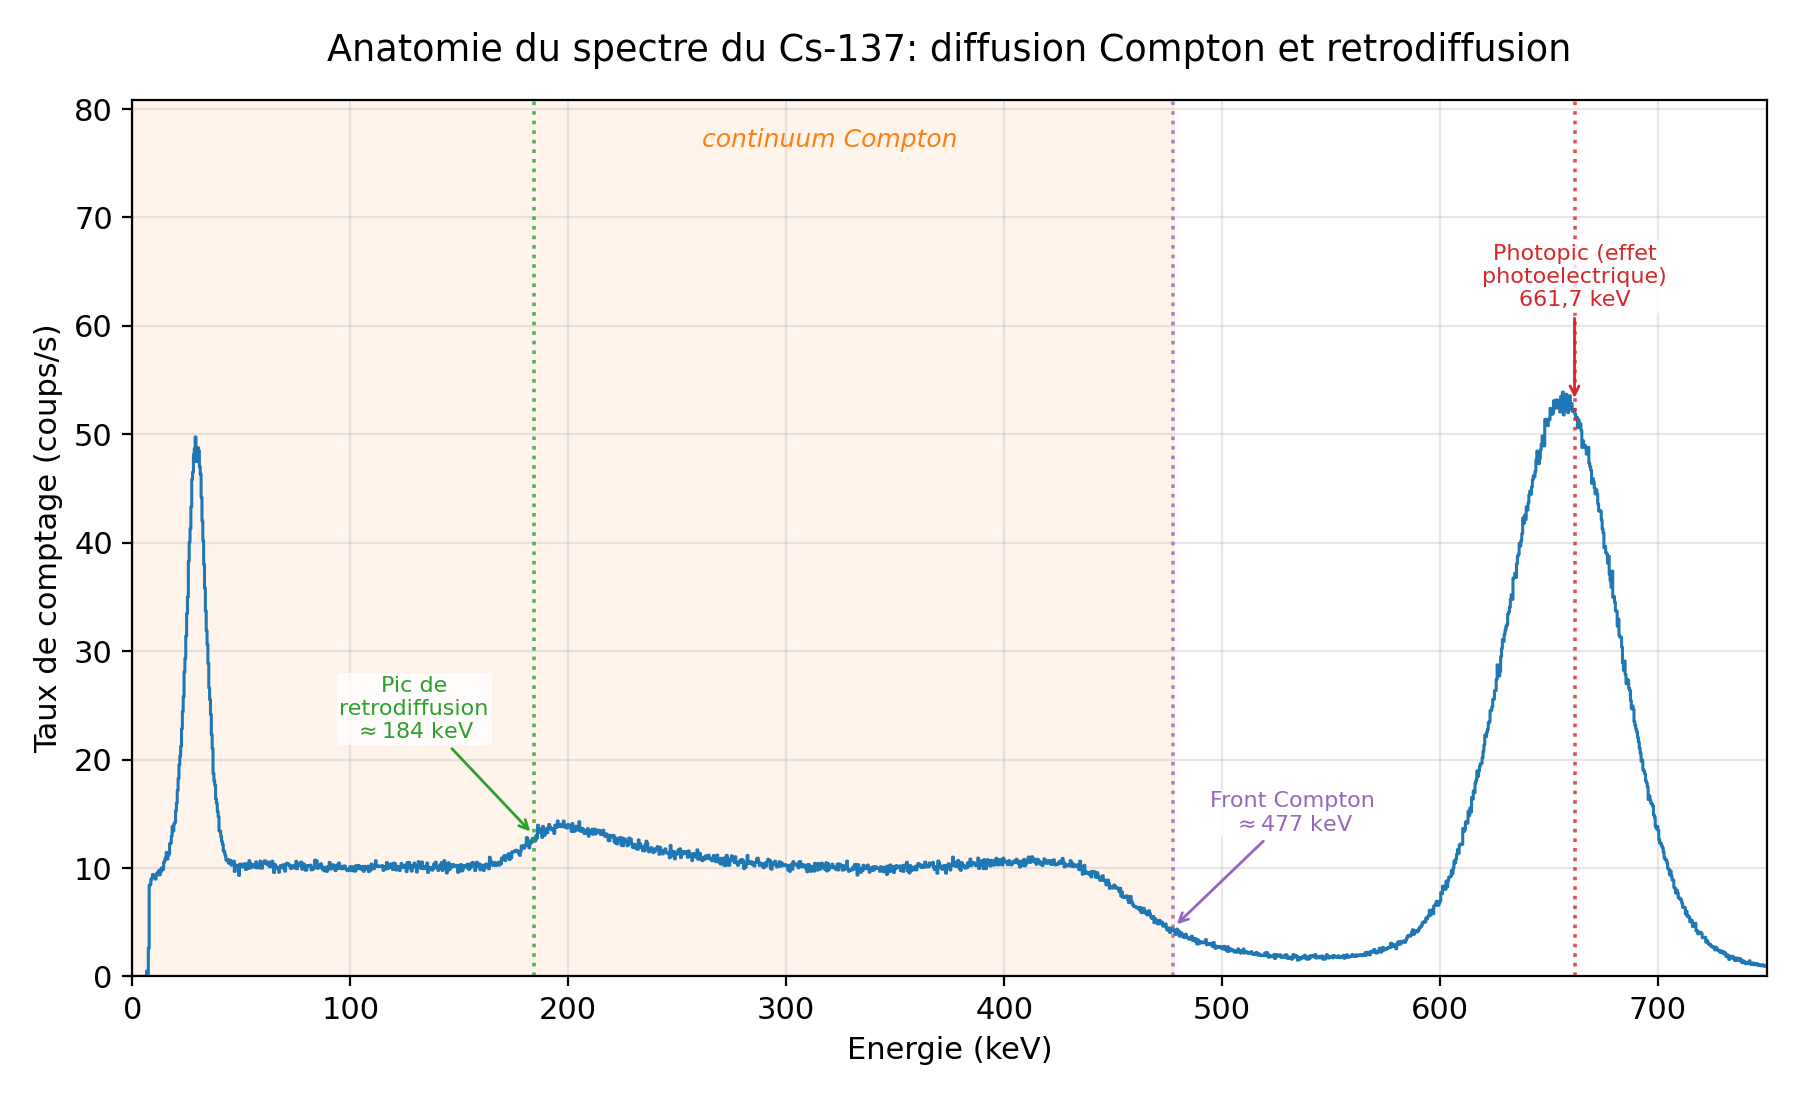
\includegraphics[width=0.85\textwidth]{../figures/09_compton_cs137.png}
    \caption{Spectre du \textsuperscript{137}Cs annoté: le photopic (effet photoélectrique), le front Compton et le pic de rétrodiffusion prédits par la cinématique de la diffusion Compton coïncident avec les structures observées, à la résolution du détecteur près. La zone ombragée délimite le continuum Compton, sous le front théorique.}
    \label{fig:compton}
\end{figure}

\subsection{Résolution en énergie}

La résolution relative $R = \text{FWHM}/E$ de chaque photopic (Tableau~\ref{tab:peaks}) diminue systématiquement avec l'énergie, d'environ 28 à 34~\% pour les raies sous 35~keV jusqu'à environ 4,5 à 5~\% pour les raies du \textsuperscript{60}Co au-delà de 1,1~MeV (Figure~\ref{fig:resolution}). Un ajustement en loi de puissance donne
\beq{eq:resolution}
    R(E) = (122 \pm 15) \cdot E^{-0,44 \pm 0,03}~\% \quad (E \text{ en keV}) ,
\enq
proche de la dépendance $E^{-1/2}$ attendue pour un détecteur limité par la statistique de comptage des photons de scintillation \cite{knoll}.

\begin{figure}[H]
    \centering
    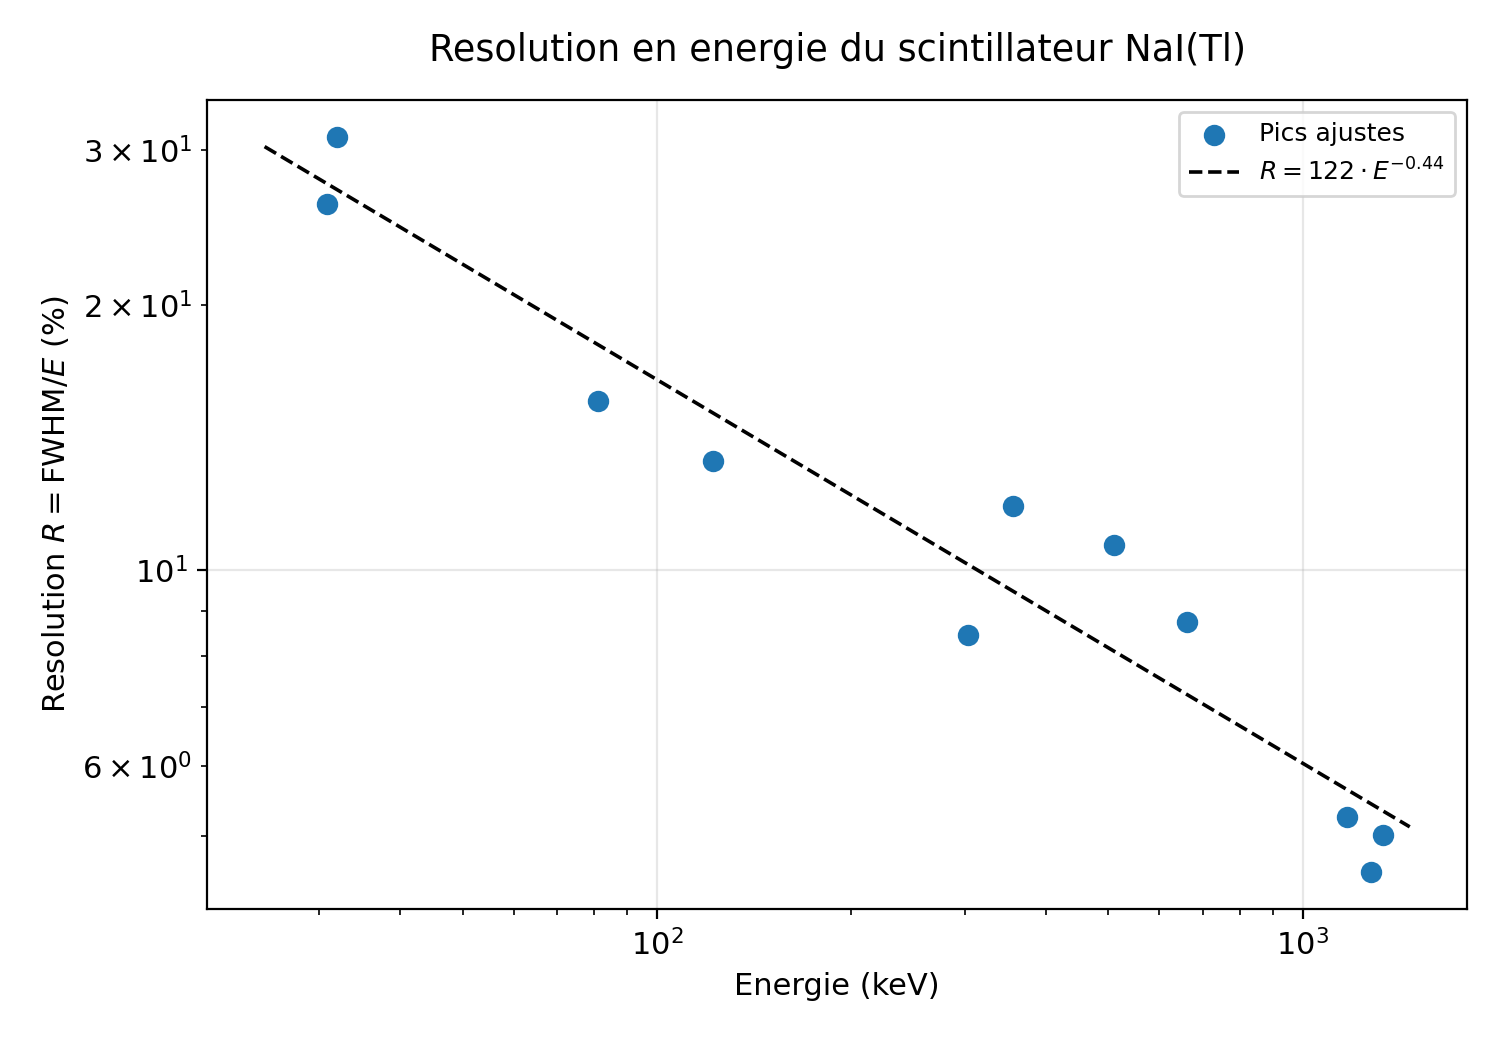
\includegraphics[width=0.68\textwidth]{../figures/10_resolution.png}
    \caption{Résolution en énergie du scintillateur en fonction de l'énergie, pour les onze photopics ajustés. L'exposant mesuré ($-0,44$) est proche de la valeur $-0,5$ attendue pour un régime dominé par le bruit statistique de comptage des photons.}
    \label{fig:resolution}
\end{figure}

\subsection{Identification du bruit de fond ambiant}

Le spectre du bruit de fond (Figure~\ref{fig:background}), accumulé sur 36~minutes en l'absence de toute source, montre un continuum qui décroît globalement avec l'énergie, la superposition des continuums Compton de multiples émetteurs naturels et du rayonnement cosmique, surmonté d'une bosse nette entre $\sim 1350$ et $\sim 1550$~keV. Un ajustement gaussien de cette structure situe son centroïde à $1485 \pm 3~\text{keV}$, à comparer à la raie de référence du \textsuperscript{40}K à $1460,8~\text{keV}$ \cite{nndc}. C'est la seule raie intense attendue dans cette gamme d'énergie pour un environnement de laboratoire typique, et sa position est conforme à l'indice donné dans le protocole, qui situe la principale source de radioactivité ambiante entre 1400 et 1500~keV \cite{protocole}.

\begin{figure}[H]
    \centering
    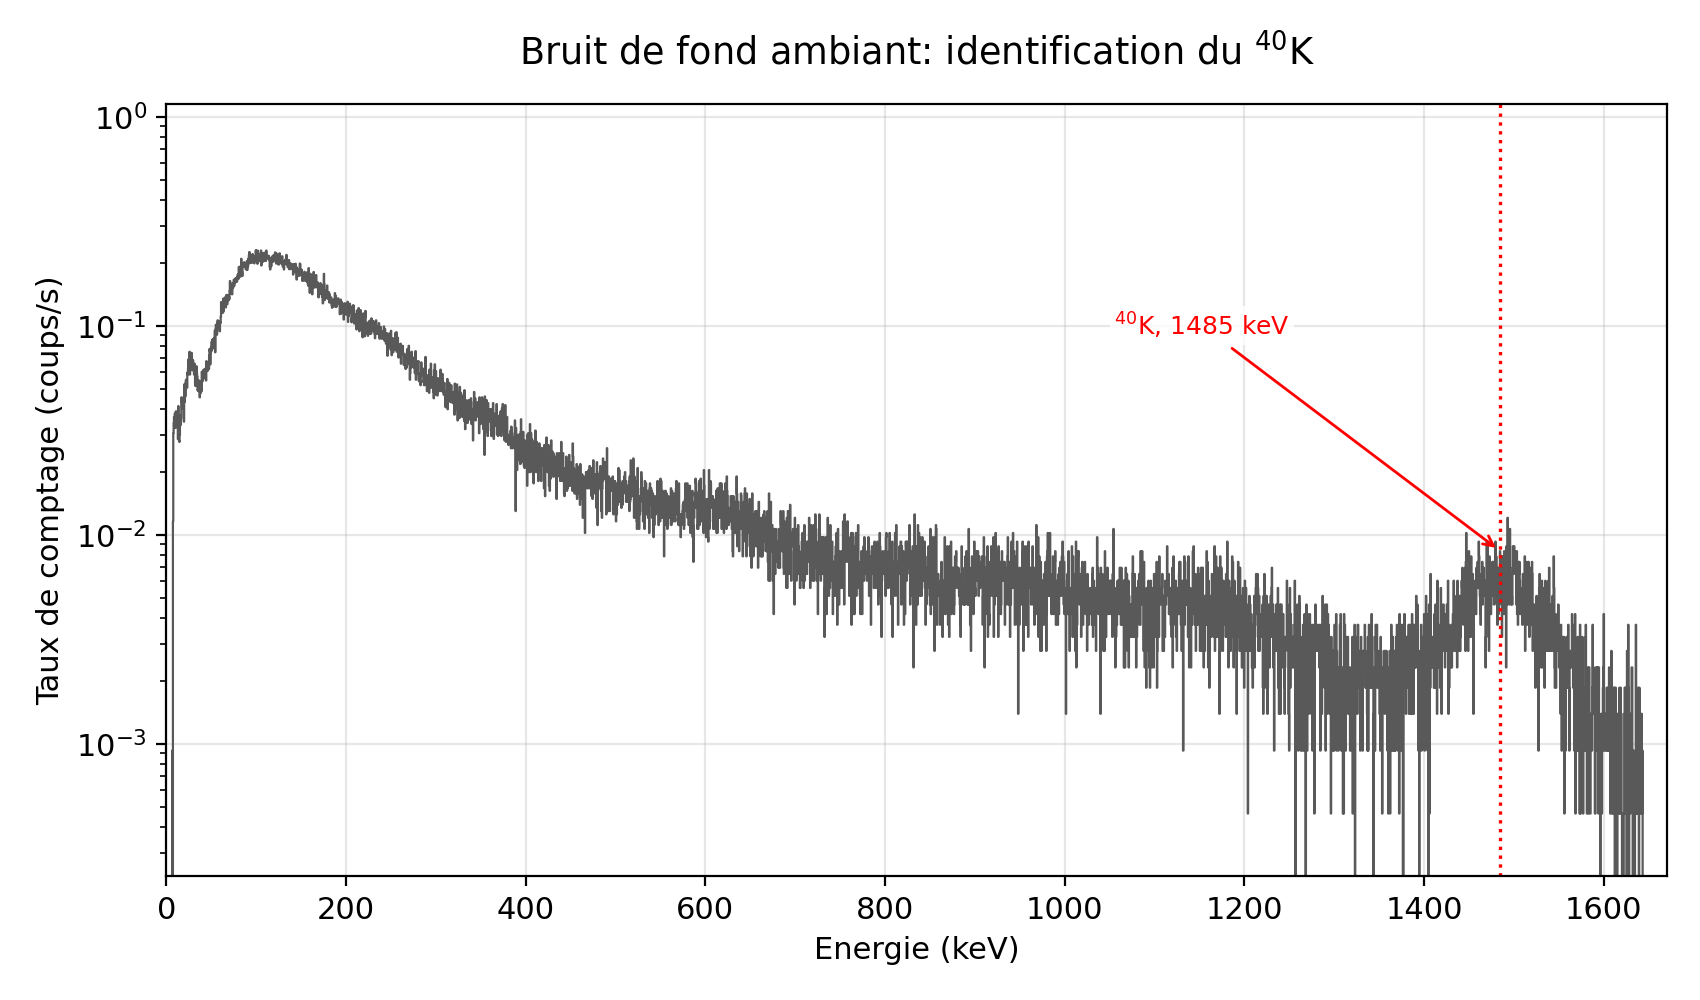
\includegraphics[width=0.78\textwidth]{../figures/08_background_K40.png}
    \caption{Spectre du bruit de fond ambiant (échelle logarithmique, 36~minutes d'acquisition). La raie identifiée à $1485 \pm 3~\text{keV}$ est attribuée au \textsuperscript{40}K (1460,8~keV), présent naturellement dans le béton, la brique et le corps humain.}
    \label{fig:background}
\end{figure}

\section{Discussion}

\subsubsection*{Qualité de l'étalonnage}
Le choix du modèle quadratique plutôt que linéaire est appuyé quantitativement (RMSE réduit de près de moitié) et qualitativement (les résidus du modèle linéaire montrent une courbure systématique, typique d'un défaut de linéarité du couple PM/amplificateur aux basses énergies, bien documenté dans la littérature \cite{knoll}). Les résidus individuels du Tableau~\ref{tab:peaks} restent tous inférieurs à 5~keV, cohérents avec le RMSE global. Aucune source ne se démarque par un biais systématique, ce qui suggère que l'erreur dominante est bien la non-linéarité résiduelle du détecteur plutôt qu'une erreur d'identification de raie propre à une source.

\subsubsection*{Incertitudes}
Les incertitudes statistiques sur les centroïdes ajustés (issues de la matrice de covariance du fit gaussien, Tableau~\ref{tab:peaks}) sont systématiquement plus petites, souvent de un à deux ordres de grandeur, que les résidus du modèle d'étalonnage. Autrement dit, ce n'est pas le bruit de comptage qui limite la précision de notre étalonnage, mais bien des effets systématiques: légère dérive de linéarité, largeur finie des raies qui rend le centroïde sensible à la forme exacte du fond sous le pic, et pour les deux raies sous 35~keV, la proximité du seuil d'absorption K de l'iode ($\sim 33,2~\text{keV}$), où la section efficace photoélectrique du NaI varie brusquement et déforme le pic. Ceci offre une explication plausible à leur résolution nettement moins bonne (28~\% et 34~\%) que ne le prédit la tendance générale en $E^{-0,44}$ (Figure~\ref{fig:resolution}).

\subsubsection*{Front Compton et rétrodiffusion}
L'accord entre les positions prédites et mesurées (Section~4.2) confirme que la cinématique de diffusion Compton à un seul choc décrit bien la physique en jeu, et que les écarts résiduels ($\sim 15$~keV pour le front, $\sim 11$~keV pour la rétrodiffusion) sont pleinement explicables par la résolution finie du détecteur, qui « étale » ces structures normalement abruptes sur une largeur comparable au FWHM local. Ce test est en un sens plus exigeant que l'étalonnage lui-même: il ne repose sur aucun point ajusté, seulement sur la physique de la diffusion Compton appliquée à une énergie de raie connue indépendamment.

\subsubsection*{Identification du \textsuperscript{40}K}
L'écart entre la valeur mesurée ($1485 \pm 3~\text{keV}$) et la valeur de référence ($1460,8~\text{keV}$) est de $24~\text{keV}$, soit environ un écart-type de la largeur du pic à cette énergie ($\sigma \approx \text{FWHM}/2,35 \approx 31~\text{keV}$, d'après l'équation~\ref{eq:resolution}). L'identification demeure donc solide, mais l'écart est plus grand que pour les raies d'étalonnage elles-mêmes. L'explication la plus probable est que $1461~\text{keV}$ se situe au-delà de la raie d'étalonnage la plus énergétique utilisée (1332,5~keV, \textsuperscript{60}Co): le modèle quadratique extrapole donc légèrement hors de son domaine de validation à cette énergie, ce qui est une limite connue de ce genre d'ajustement. Une source de \textsuperscript{40}K ou une autre source proche de 1461~keV n'était toutefois pas disponible pour ancrer directement l'étalonnage à cette énergie.

\subsubsection*{Limites et améliorations}
Le montage utilisé ne permet pas de mesurer une activité absolue (aucune information sur la distance source-détecteur ni sur l'angle solide n'a été consignée durant la manipulation, celle-ci n'étant pas nécessaire pour un étalonnage en énergie). Une prochaine itération de l'expérience gagnerait à documenter systématiquement la géométrie pour permettre, en plus de l'identification, une estimation quantitative de l'activité des sources. La résolution modeste du NaI(Tl) (comparée par exemple à un détecteur au germanium hyperpur) limite aussi la capacité à distinguer des raies proches en énergie. Un détecteur HPGe aurait permis de résoudre plus finement la région du \textsuperscript{40}K et de vérifier la présence, ou l'absence, des raies plus faibles des chaînes de l'uranium et du thorium, généralement en dessous du bruit statistique ici. Enfin, une acquisition de bruit de fond plus longue (au-delà de 36~minutes) réduirait l'incertitude statistique sur la position du pic de \textsuperscript{40}K et permettrait de confirmer sa position avec plus de confiance.

\section{Conclusion}

Le scintillateur NaI(Tl) a été étalonné avec succès à l'aide de cinq sources $\gamma$ connues, avec un modèle quadratique canal-énergie atteignant une précision de 2,6~keV (RMSE) sur une plage de 30~keV à 1,33~MeV. Les deux objectifs de l'expérience ont été atteints: l'instrument calibré a permis de vérifier quantitativement la physique de la diffusion Compton (front Compton et pic de rétrodiffusion du \textsuperscript{137}Cs conformes aux prédictions théoriques, à la résolution près) et d'identifier la source dominante du bruit de fond ambiant du laboratoire comme étant le \textsuperscript{40}K, avec une énergie mesurée en accord avec la valeur de référence à moins d'un écart-type. Au passage, la résolution en énergie du détecteur a été caractérisée sur plus d'un ordre de grandeur en énergie, révélant un comportement proche du régime limité par la statistique de comptage des photons de scintillation ($R \propto E^{-0,44}$, contre $E^{-0,5}$ attendu).

Cette même démarche, étalonner un détecteur puis identifier une source à partir de son spectre, est utilisée par exemple dans les portiques de détection radiologique aux frontières, la surveillance environnementale autour de centrales nucléaires, ou l'identification de contaminants en médecine nucléaire. Dans notre cas, ce bruit de fond a permis d'identifier une source réelle de radioactivité présente dans l'environnement du laboratoire, plutôt que d'être simplement écarté comme signal parasite.

\renewcommand{\refname}{Bibliographie}
\begin{thebibliography}{9}

\bibitem{knoll}
Knoll, G.F. \textit{Radiation Detection and Measurement}, 4\textsuperscript{e} édition. John Wiley \& Sons, 2010.

\bibitem{bevington}
Bevington, P.R. \& Robinson, D.K. \textit{Data Reduction and Error Analysis for the Physical Sciences}, 3\textsuperscript{e} édition. McGraw-Hill, 2002.

\bibitem{nndc}
National Nuclear Data Center, Brookhaven National Laboratory. \textit{NuDat 3.0: Nuclear Structure and Decay Data}. \url{https://www.nndc.bnl.gov/nudat3/} (données du \textsuperscript{40}K, \textsuperscript{133}Ba, \textsuperscript{57}Co, \textsuperscript{60}Co, \textsuperscript{137}Cs, \textsuperscript{22}Na).

\bibitem{protocole}
Département de physique, de génie physique et d'optique, Université Laval. \textit{GPH-3000, Travaux pratiques avancés: Détecteurs de radiations nucléaires}, version 2019-09-23, et \textit{Résumé des manipulations}, version 2022-09-22.

\end{thebibliography}

\section*{Annexe: spectres individuels des sources d'étalonnage}

Les quatre figures suivantes montrent les spectres complets des sources utilisées pour l'étalonnage (à l'exception du \textsuperscript{137}Cs, présenté en détail à la Figure~\ref{fig:compton}), avec les raies de référence identifiées. Elles sont fournies à titre complémentaire. Le corps du rapport est compréhensible sans s'y référer.

\begin{figure}[H]
    \centering
    
\includegraphics[width=0.72\textwidth]{../figures/02_spectre_Ba133.png}
    \caption{Spectre du \textsuperscript{133}Ba, quatre raies de référence de 30,85 à 356,02~keV.}
\end{figure}

\begin{figure}[H]
    \centering
    
\includegraphics[width=0.72\textwidth]{../figures/03_spectre_Co57.png}
    \caption{Spectre du \textsuperscript{57}Co, raie unique à 122,06~keV.}
\end{figure}

\begin{figure}[H]
    \centering
    
\includegraphics[width=0.72\textwidth]{../figures/04_spectre_Co60.png}
    \caption{Spectre du \textsuperscript{60}Co, doublet caractéristique à 1173,20 et 1332,50~keV.}
\end{figure}

\begin{figure}[H]
    \centering
    
\includegraphics[width=0.72\textwidth]{../figures/06_spectre_Na22.png}
    \caption{Spectre du \textsuperscript{22}Na, incluant le pic d'annihilation à 511,00~keV et la raie nucléaire à 1274,50~keV.}
\end{figure}

\end{document}
